
\subsubsection{UC1 - Visualizzazione activity introduttiva}
\begin{itemize}
	\item \textbf{Attori Primari}: utente generico;
	\item \textbf{Descrizione}: l'utente visualizza visualizza la pagina iniziale da cui è possibile raggiungere l'activity\glosp di login e l'activity di registrazione;
	\item \textbf{Scenario principale}: l'utente accede all'activity introduttiva dell'applicazione e può decidere se registrarsi o effettuare l'accesso;
	\item \textbf{Precondizione}: il sistema è raggiungibile e funzionante, l'utente accede all'activity iniziale dell'applicazione;
	\item \textbf{Postcondizione}: il sistema fornisce all'utente, la possibilità di raggiungere l'activity di login o quella di registrazione.
	
	
\end{itemize}
\subsubsection{UC2 - Registrazione}
\begin{figure}[h]
	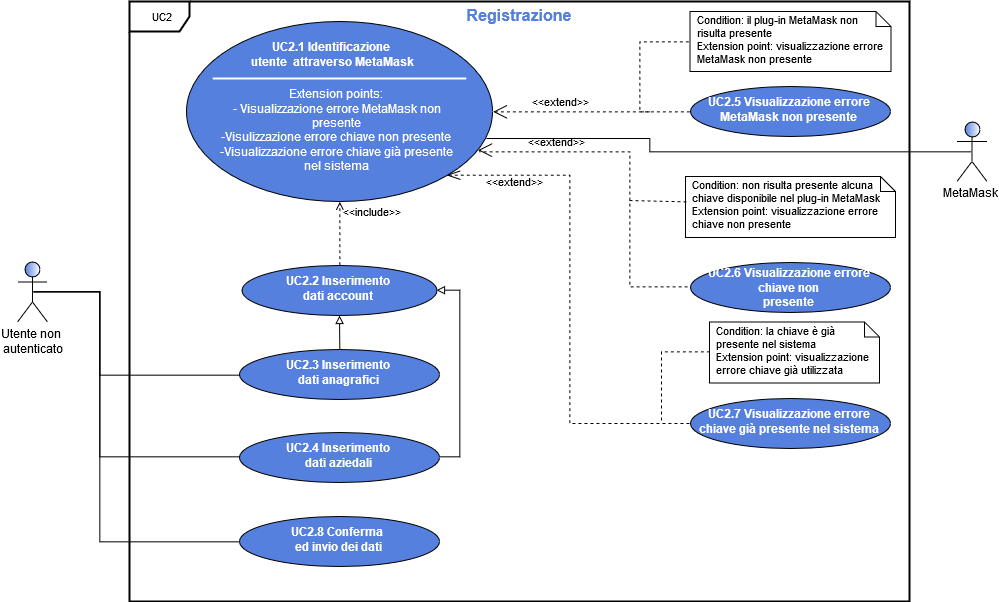
\includegraphics[width=9cm]{res/images/UC2Registrazione.png}
	\centering
	\caption{UC2 - Registrazione}
\end{figure}
\begin{itemize}
	\item \textbf{Attori Primari}: utente non autenticato;
	%\item \textbf{Attori Secondari}: Movens\glo;
	\item \textbf{Descrizione}: per effettuare il procedimento di registrazione, l'utente deve compilare tutti i campi necessari ovvero nome, cognome, email e password;
	\item \textbf{Scenario principale}: l'applicazione rende disponibili i campi da compilare per la registrazione. Dunque l'utente dovrà inserire tutti i dati necessari.
		
	\item \textbf{Precondizione}: l'utente ha inserito correttamente tutti i dati necessari nei campi.
	\item \textbf{Postcondizione}: dopo aver controllato attraverso la piattaforma Movens che i campi sono stati compilati correttamente, l'utente viene registrato nell'applicazione. 
	
\end{itemize}
\subsubsection{UC2.1 - Inserimento dati profilo utente}
\begin{itemize}
	\item \textbf{Attori Primari}: utente non autenticato;
	\item \textbf{Descrizione}:l'utente compila i campi contenenti i dati relativi al profilo utente;
	\item \textbf{Scenario principale}: l'utente compila tutti i campi del form riguardanti l'account, ovvero:
	a.l'utente inserisce il proprio nome [UC2.1.1];
	\newline
	b.l'utente inserisce il proprio cognome [UC2.1.2];
	\newline
	c.l'utente inserisce l'email da associare all'account [UC2.1.3];
	\newline
	d.l'utente inserisce la password da associare all'account [UC2.1.4].
	\item \textbf{Precondizione}: l'utente è entrato nell'activity di registrazione;
	\item \textbf{Postcondizione}: l'utente ha compilato tutti i campi richiesti dalla registrazione.
\end{itemize}
\begin{figure}[h]
	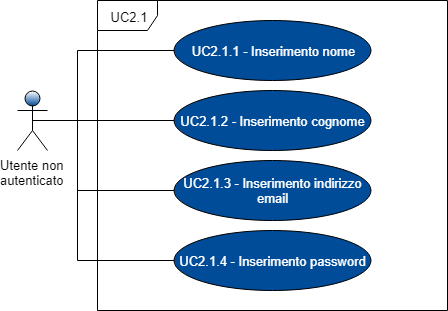
\includegraphics[width=9cm]{res/images/UC2-1Inserimento.png}
	\centering
	\caption{UC2.1 - Inserimento dati profilo utente}
\end{figure}
\subsubsection{UC2.1.1 - Inserimento nome}
\begin{itemize}
	\item \textbf{Attori Primari}: utente non autenticato;
	\item \textbf{Descrizione}: al fine di portare a termine il processo di registrazione l'utente deve inserire il proprio nome, campo ritenuto obbligatorio;
	\item \textbf{Scenario principale}: l'utente compila il campo relativo al nome;	
	\item \textbf{Precondizione}: l'applicazione ha reso disponibile il campo per l'inserimento del nome;
	\item \textbf{Postcondizione}: l'utente ha compilato il campo con il proprio nome.	
\end{itemize}
\subsubsection{UC2.1.2 - Inserimento cognome}
\begin{itemize}
	\item \textbf{Attori Primari}: utente non autenticato;
	\item \textbf{Descrizione}: al fine di portare a termine il processo di registrazione l'utente deve inserire il proprio cognome, campo ritenuto obbligatorio;
	\item \textbf{Scenario principale}: l'utente compila il campo relativo al cognome;	
	\item \textbf{Precondizione}: l'applicazione ha reso disponibile il campo per l'inserimento del cognome;
	\item \textbf{Postcondizione}: l'utente ha compilato il campo con il proprio cognome.	
\end{itemize}
\subsubsection{UC2.1.3 - Inserimento indirizzo e-mail}
\begin{itemize}
	\item \textbf{Attori Primari}: utente non autenticato;
	\item \textbf{Descrizione}: al fine di portare a termine il processo di registrazione l'utente deve inserire il proprio indirizzo e-mail, campo ritenuto obbligatorio;
	\item \textbf{Scenario principale}: l'utente compila il campo relativo all'indirizzo e-mail;	
	\item \textbf{Precondizione}: l'applicazione ha reso disponibile il campo per l'inserimento dell'indirizzo e-mail;
	\item \textbf{Postcondizione}: l'utente ha compilato il campo con il proprio indirizzo e-mail.
\end{itemize}
\subsubsection{UC2.1.4 - Inserimento password}
\begin{itemize}
	\item \textbf{Attori Primari}: utente non autenticato;
	\item \textbf{Descrizione}: al fine di portare a termine il processo di registrazione l'utente deve inserire una password, campo ritenuto obbligatorio;
	\item \textbf{Scenario principale}: l'utente compila il campo relativo alla password;	
	\item \textbf{Precondizione}: l'applicazione ha reso disponibile il campo per l'inserimento della password;
	\item \textbf{Postcondizione}: l'utente ha compilato il campo con una password.
\end{itemize}
\subsubsection{UC2.2 - Invio dati}
\begin{itemize}
	\item \textbf{Attori Primari}: utente non autenticato;
	\item \textbf{Descrizione}: l'utente preme il pulsante per la conferma e l'invio dei dati; l'utente verrà rimandato a una nuova activity che confermerà il successo dell'operazione.
	\item \textbf{Scenario principale}: l'utente preme il pulsante di verifica ed invio dei dati;	
	\item \textbf{Precondizione}: i campi dati necessari per la registrazione sono compilabili. È presente il pulsante per la conferma dei dati;
	\item \textbf{Postcondizione}: l'utente viene rimandato a una nuova activity che conferma il successo dell'operazione e avvisa l'utente di controllare la propria e-mail per confermare il processo di registrazione.
\end{itemize}


